\chapter{Implementing the System}

	In the following chapter, the overall design of the system is discussed. First and foremost, the basic architecture and development platform will be decided, before moving into more technical aspects of designing the software.


	\section{The Architecture}
		Since it's already been determined, that the resulting product is something which should be found in the private cloud, it seems obvious that a Web UI is needed.

		To achieve this, there is a plethora of various languages and tools available, to aid in development of such software. However, since the aim is to create a solution which is able to run on almost any platform, technologies such as Microsoft's IIS, ASP.NET and the lot is automatically excluded.



		Since it is a web application being developed, the basic architecture can be split up into two groups: Front-end and back-end.

		\subsection{The Back-End}
			When creating web applications there are two primary ways of doing it: Creating a API-centric web application, or creating an "old fashioned" web application.

			The advantage of creating a API-centric web application, is that the back end is re-usable, for clients on other platforms. For instance, a native client on Windows, a website, and a browser plugin can all use the same API, thus removing the need of developing a back-end for each platform.

			This alone, is sufficient reason enough to choose to create an API-centric web app, simply due to keeping future possibilities open.

			When developing a web application, there are numerous different languages and tools available. make
			Web development seems to be centered around four languages, as seen on the list further down. Note that ASP.NET has purposefully been excluded from this list, due to it running only on Microsoft platforms, which is in conflict with the requirements.
			
			\begin{itemize}
				\item PHP
				\item JavaScript
				\item Ruby
				\item Python
			\end{itemize}

			\subsubsection{The Language}

				Some developers argue that choosing between languages is primarily up to personal preference. Additionally, language choice can often be effected by existing technologies used in a company. In this case, however, it's a clean slate. No prior work has been done, and the choice is as such not influenced by this.

				As an astute reader might see, JavaScript makes an appearance on this list. While previously, JavaScript was a front-end only language, with the introduction of Node.JS \todo{Node.JS URL}, around the year 2009, this changed. Suddenly JavaScript was a viable contender for use as a back-end language.

				Looking at GitHub's language trends as of August 19, 2015 \footnote{https://github.com/blog/2047-language-trends-on-github} it is clear that while both Python and Ruby have declined, JavaScript has risen on popularity. However, this graph should not be taken as gospel, at least not completely. It only shows popularity of languages used in repositories hosted on GitHub.

				The following few subsections, will contain a brief description and comparison of the languages.

				\paragraph{PHP}
					PHP is probably the the old and tested, of the languages listed previously. It has existed for ages, and is currently on version 7.



				\paragraph{JavaScript w. NodeJS}
					While Node.JS stricly speaking only supports a single thread \emph{(unless using the Cluster\footnote{https://nodejs.org/api/cluster.html} module)}, it handles massive amount of traffic easily.

					Node.JS is built using Chrome's V8 JavaScript engine, and is centered around non-blocking I/O, resulting in optimal usage of that one single thread.

					An advantage of Node, is that you can use the same language for front-end and back-end. The JavaScript written for the browser, is virtually no different from the one used in Node for a back-end. 
				\paragraph{Ruby}
				\paragraph{Python}


		\subsection{The Database}

		\subsection{The Front-End}

		\subsection{How It Ties Together}

	\section{Testing}
	zz

	\section{Encryption Schemes}
	\section{Database Design}

	\section{Authentication}
		Satellizer: https://github.com/sahat/satellizer/blob/master/examples/server/node/server.js\\

		For securing your API there are a few different approaches.

		Cookies vs Token Based

		Since it would be preferable to keep the options of down the road, creating native clients and possibly browser plugins, a token based authentication scheme is preferable, as cookies will only present more trouble at that time.

		First and foremost, generally speaking an API key is preferable over the user of username and password. However, in this case it is suboptimal, since the user will be logging on on a website.

		The two obvious approaches is using either OAuth 1.0A or OAuth2. However, both of these require either using a third party to login, i.e. Google or Facebook, or implementing a OAuth provider in Ghost. This is not desirable, due to the requirements of creating new users, and simply due to privacy issues.

		That leaves a local solution. The most prominent approach to this, is to use the JSON Web Tokens \emph{(JWT)} described in \cite{JWT}. However, for this to be secure \emph{all} communication must happen over TLS. Due to the nature of the project, this was already a requirement.

		

	\section{The Frameworks}
			\subsubsection{The Framework}
			Having decided on using JavaScript and Node.JS for the web applications back-end, the next thing that needs to be determined is which back-end framework to use -- if any at all!

			Strictly speaking, Node.JS has the tools built in to work as a web-server already. It already has methods and modules for creating a RESTful API. However, it is a very crude setup. Frameworks such as the popular Express aid in the development of these APIs, making giving the developer tools at his or her disposal, to test, debug, and develop. The following list, contains the frameworks centered around exposing a RESTful API.

			\begin{itemize}
				\item Express
				\item Restify
				\item Hapi
			\end{itemize}

			While there exists plenty of more tools, that what is written on this list, they primarily focus on not only supplying the framework for development, but also for templating. This results in their usage is generally more towards ``old fashioned'' web application.

			Frameworks such as Express and Restify, however, focus on building an API around which the application is centered. It is exactly this type of tool, which is needed for the purpose of this project.

			While Express seems to be the default choice when it comes to Node, it has some	drawbacks. First and foremost, Express had some internal drama in 2014, where the original developer ``sold'' the Express framework, to StrongLoop \todo{Source: http://gilesbowkett.blogspot.dk/2014/07/the-bizarre-bazaar-who-owns-expressjs.html }. Since StrongLoop is a company whose commercial strategy relies on Express, this might end up resulting in some issues down the line. Additionally, Express have a lot of features not necessarily required for this project, which might result in some bloat. Finally, its seen on figure \ref{fig:node_performance} on page \pageref{fig:node_performance} that while Express' is better than that of Hapi, it is still inferior to that of Restify. The advantage, however, is that Express is currently the most used and battle tested. As such more information is readily available online. It is less unlikely, that no one else has encountered any given problem previously.

			Restify on the other hand, is a lightweight framework built with one and only purpose: Exposing an RESTful API. This speed is evident from figure \ref{fig:node_performance} where it beats not only Express but also Hapi, in number of requests per second. However, this advantage seems to stem from the fact that apparently Restify keeps connections alive, which reduces overhead in the creation of connections. Unfortunately, since it is a smaller framework, the amount of information is reduced in comparison to Express.

			
			Hapi is the last framework from the list. Developed by Walmart Labs, Hapi claims to take a slightly different route than the previous two: It focusses more on application logic. 

			\begin{figure}[htbp]
				\centering
				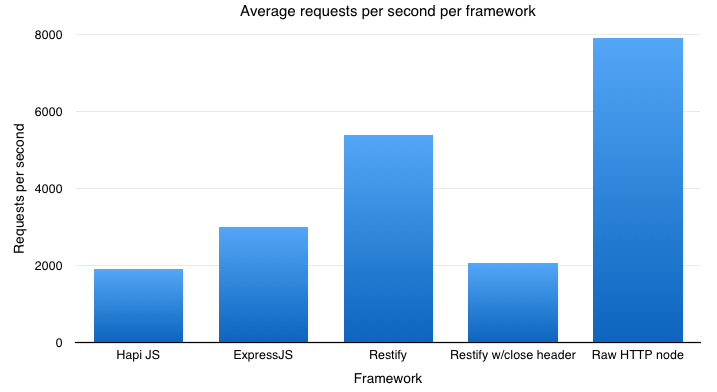
\includegraphics[width=0.95\textwidth]{figures/design/node-framework-performance.png}
				\caption{Performance comparison of Node.JS web frameworks, courtesy of Raygun Labs \cite{node_framework}}
				\label{fig:node_performance}
			\end{figure}